\documentclass[10pt,a4paper]{article}

% ===================== PAQUETES =====================
\usepackage[utf8]{inputenc}
\usepackage[spanish]{babel}
\usepackage[margin=2cm]{geometry}
\usepackage{graphicx}
\usepackage{listings}
\usepackage{xcolor}
\usepackage{tikz}
\usetikzlibrary{shapes,arrows.meta,positioning}
\usepackage{hyperref}
\usepackage{caption}
\usepackage{booktabs}
\usepackage{amsmath}
\usepackage{titlesec}
\usepackage{enumitem}
\usepackage{float}
\usepackage{placeins}

\hypersetup{colorlinks=true, linkcolor=black, urlcolor=blue, citecolor=black}

\titlespacing*{\section}{0pt}{8pt}{4pt}
\titlespacing*{\subsection}{0pt}{6pt}{2pt}
\setlist{itemsep=1pt, topsep=2pt}

\lstdefinestyle{sql}{
  language=SQL,
  basicstyle=\ttfamily\scriptsize,
  keywordstyle=\color{blue}\bfseries,
  commentstyle=\color{gray}\itshape,
  stringstyle=\color{teal},
  breaklines=true,
  frame=single,
  numbers=left,
  numberstyle=\tiny\color{gray},
  showstringspaces=false,
  aboveskip=4pt,
  belowskip=4pt
}
\lstset{style=sql}

\captionsetup{font=small,skip=3pt}
\setlength{\intextsep}{6pt}
\setlength{\textfloatsep}{8pt}

% ===================== PORTADA =====================
\title{\textbf{Diseño y fragmentación de una base de datos distribuida} \\
\large Práctica de Fragmentación Distribuida --- Sistema de Cafetería Multi-Sede}
\author{
  % TODO: reemplaza por los nombres reales del equipo
  Jeremy Ruperto Gaibor Rodriguez \\
  \\
  \textit{Ingeniería de Software --- Aplicaciones Distribuidas (ISR-701)} \\
  \textit{Universidad Técnica Estatal de Quevedo (UTEQ)}
}
\date{\today}

\begin{document}

\maketitle

% ===================== INTRODUCCIÓN =====================
\section{Introducción}

Las bases de datos distribuidas permiten repartir la información entre distintos
nodos físicos sin perder la posibilidad de consultarla como si fuera un único
sistema \cite{ozsu}. En esta práctica se diseñó un esquema de fragmentación horizontal,
vertical y mixta para el sistema de pedidos de una cafetería con tres sedes:
Campus, Babahoyo y Ventanas. El objetivo fue distribuir la información de
clientes y pedidos entre tres nodos PostgreSQL independientes, verificar que la
fragmentación cumple las propiedades de completitud, reconstrucción y
disjunción, y construir vistas globales capaces de reconstruir la información
como si estuviera centralizada, apoyándose en el módulo \texttt{postgres\_fdw}.

Este informe documenta el entorno desplegado, las decisiones de diseño tomadas
para cada tipo de fragmentación, la evidencia de ejecución obtenida mediante
\texttt{psql}, y una reflexión final sobre las ventajas y dificultades
observadas durante el desarrollo.

% ===================== C1 =====================
\section{Entorno operativo}

El entorno se construyó con \texttt{docker-compose} \cite{docker}, levantando tres
contenedores PostgreSQL independientes, uno por cada sede de la cafetería
(Campus, Babahoyo, Ventanas), cada uno con su propio volumen de datos y su
propio puerto expuesto en el host (5433, 5434 y 5435 respectivamente). Esta
separación de puertos y volúmenes garantiza que cada nodo es completamente
autónomo: no comparte disco ni proceso con los demás.

\begin{figure}[h]
  \centering
  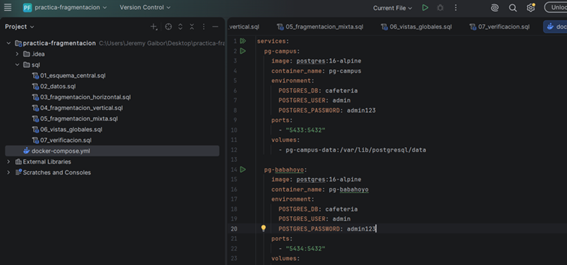
\includegraphics[width=0.6\linewidth]{imagenes/fig02_docker_compose_yml.png}
  \caption{Definición de los tres contenedores PostgreSQL en \texttt{docker-compose.yml}.}
  \label{fig:compose}
\end{figure}

Tras ejecutar \texttt{docker compose up -d}, los tres contenedores quedaron en
ejecución simultánea, lo que se confirmó con \texttt{docker compose ps}
(Figura~\ref{fig:up}).

\begin{figure}[h]
  \centering
  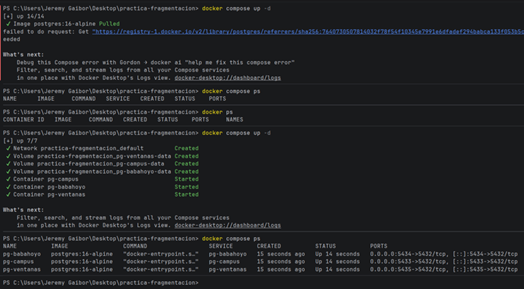
\includegraphics[width=0.6\linewidth]{imagenes/fig03_docker_compose_up.png}
  \caption{Los tres nodos levantados en segundo plano con un solo comando.}
  \label{fig:up}
\end{figure}

La conexión a cada nodo se realizó con el cliente \texttt{psql} incluido en la
propia imagen del contenedor, sin necesidad de instalar herramientas
adicionales en el host:

\begin{lstlisting}
docker exec -it pg-campus psql -U admin -d cafeteria
\end{lstlisting}

\begin{figure}[h]
  \centering
  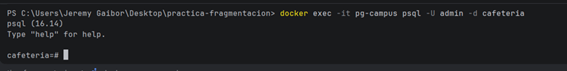
\includegraphics[width=0.6\linewidth]{imagenes/fig04_psql_conexion.png}
  \caption{Sesión \texttt{psql} abierta dentro del contenedor \texttt{pg-campus}.}
  \label{fig:psql}
\end{figure}

% ===================== C2 =====================
\section{Esquema centralizado}

Antes de fragmentar la base de datos fue necesario definir el esquema completo
en un único nodo de referencia (\texttt{pg-campus}). Este esquema centralizado
contiene las tablas \texttt{clientes}, \texttt{productos} y \texttt{pedidos},
con sus respectivas claves primarias y las claves foráneas que relacionan los
pedidos con clientes y productos.

\begin{lstlisting}
CREATE TABLE clientes (
    cliente_id SERIAL PRIMARY KEY,
    nombre     VARCHAR(80) NOT NULL,
    ciudad     VARCHAR(40) NOT NULL,
    email      VARCHAR(120) NOT NULL,
    telefono   VARCHAR(20)
);

CREATE TABLE productos (
    producto_id SERIAL PRIMARY KEY,
    nombre      VARCHAR(80) NOT NULL,
    categoria   VARCHAR(30) NOT NULL,
    precio      NUMERIC(6,2) NOT NULL CHECK (precio >= 0)
);

CREATE TABLE pedidos (
    pedido_id   SERIAL PRIMARY KEY,
    cliente_id  INTEGER NOT NULL REFERENCES clientes(cliente_id),
    producto_id INTEGER NOT NULL REFERENCES productos(producto_id),
    fecha       DATE NOT NULL,
    monto       NUMERIC(8,2) NOT NULL CHECK (monto >= 0),
    sede        VARCHAR(20) NOT NULL
);
\end{lstlisting}

El script se aplicó con:

\begin{lstlisting}
docker exec -i pg-campus psql -U admin -d cafeteria < sql/01_esquema_central.sql
\end{lstlisting}

\begin{figure}[h]
  \centering
  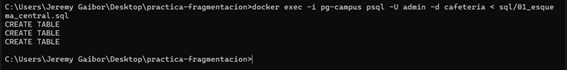
\includegraphics[width=0.6\linewidth]{imagenes/fig06_aplicar_esquema_central.png}
  \caption{Ejecución sin errores de \texttt{01\_esquema\_central.sql} en \texttt{pg-campus}.}
  \label{fig:esquema}
\end{figure}

Posteriormente se cargaron los datos de prueba (6 clientes, 5 productos y 8
pedidos) mediante \texttt{sql/02\_datos.sql}, que sirvieron como base para
todo el proceso de fragmentación posterior.

% ===================== C3 =====================
\section{Fragmentación horizontal}

La tabla \texttt{pedidos} se fragmentó horizontalmente usando la columna
\texttt{sede} como criterio de partición: cada nodo recibe únicamente las
filas cuya sede coincide con la sede física del contenedor. De los 8 pedidos
totales, 3 corresponden a Campus, 3 a Babahoyo y 2 a Ventanas.

\begin{lstlisting}
-- Ejemplo para pg-babahoyo: solo se insertan los pedidos con sede='Babahoyo'
CREATE TABLE pedidos (
    pedido_id   INTEGER PRIMARY KEY,
    cliente_id  INTEGER NOT NULL,
    producto_id INTEGER NOT NULL,
    fecha       DATE NOT NULL,
    monto       NUMERIC(8,2) NOT NULL,
    sede        VARCHAR(20) NOT NULL
);

INSERT INTO pedidos VALUES
    (2, 2, 3, '2026-03-01', 2.50, 'Babahoyo'),
    (6, 6, 1, '2026-03-03', 0.75, 'Babahoyo'),
    (8, 2, 2, '2026-03-04', 1.00, 'Babahoyo');
\end{lstlisting}

Este mismo patrón se repitió en \texttt{pg-campus} y \texttt{pg-ventanas},
filtrando cada vez por su propia sede. Con esto se garantiza \textbf{disjunción}
(ningún pedido aparece en dos nodos) y, al sumar las filas de los tres nodos,
se recupera el total original, lo que garantiza \textbf{completitud}.

% ===================== C4 =====================
\section{Fragmentación vertical}

Para la fragmentación vertical se dividió la tabla \texttt{clientes} en dos
fragmentos según la sensibilidad de la información:

\begin{itemize}
  \item \texttt{clientes\_publicos} (\texttt{cliente\_id}, \texttt{nombre},
        \texttt{ciudad}) alojado en \texttt{pg-campus}.
  \item \texttt{clientes\_contacto} (\texttt{cliente\_id}, \texttt{email},
        \texttt{telefono}) alojado en \texttt{pg-babahoyo}.
\end{itemize}

En ambos fragmentos se conserva \texttt{cliente\_id} como clave primaria
replicada, lo que permite reconstruir cualquier registro completo mediante un
\texttt{JOIN} por esa clave.

\begin{figure}[h]
  \centering
  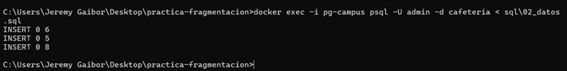
\includegraphics[width=0.6\linewidth]{imagenes/fig08_clientes_publicos_campus.png}
  \caption{Creación y carga de \texttt{clientes\_publicos} en \texttt{pg-campus}.}
  \label{fig:vpub}
\end{figure}

\begin{figure}[h]
  \centering
  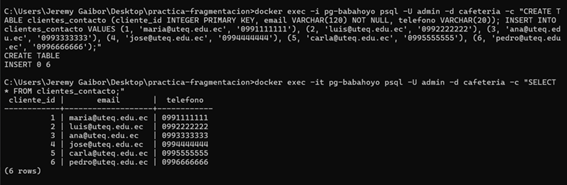
\includegraphics[width=0.6\linewidth]{imagenes/fig09_clientes_contacto_babahoyo.png}
  \caption{Creación y carga de \texttt{clientes\_contacto} en \texttt{pg-babahoyo}.}
  \label{fig:vcon}
\end{figure}

% ===================== C5 =====================
\section{Fragmentación mixta}

El diseño mixto combina ambas técnicas sobre la tabla \texttt{clientes}:
primero se particiona horizontalmente por ciudad (Quevedo frente a
Babahoyo/Ventanas) y, dentro de cada partición, se vuelve a dividir
verticalmente entre datos públicos y datos de contacto. El resultado se
resume en la Tabla~\ref{tab:mixta}.

\begin{table}[h]
  \centering
  \caption{Distribución de los fragmentos mixtos de \texttt{clientes} por nodo.}
  \label{tab:mixta}
  \begin{tabular}{@{}llll@{}}
    \toprule
    Bloque & Nodo & Fragmento & Filas (cliente\_id) \\
    \midrule
    1 & pg-campus   & \texttt{clientes\_publicos\_quevedo} & 1, 3 \\
    2 & pg-babahoyo & \texttt{clientes\_contacto\_quevedo} & 1, 3 \\
    3 & pg-ventanas & \texttt{clientes\_publicos\_otros}   & 2, 4, 5, 6 \\
    4 & pg-babahoyo & \texttt{clientes\_contacto\_otros}   & 2, 4, 5, 6 \\
    \bottomrule
  \end{tabular}
\end{table}

La Figura~\ref{fig:mixta_diagrama} adapta el esquema de fragmentación mixta a
los datos reales manejados en esta práctica.

\begin{figure}[h]
  \centering
  \begin{tikzpicture}[
      node distance=1.1cm and 1.6cm,
      nodo/.style={draw, rounded corners, fill=blue!8, minimum width=3.6cm, minimum height=1cm, align=center, font=\small},
      frag/.style={draw, rounded corners, fill=orange!12, minimum width=3.6cm, minimum height=0.9cm, align=center, font=\scriptsize}
    ]
    \node[nodo] (campus) {\textbf{pg-campus}};
    \node[nodo, right=3.2cm of campus] (babahoyo) {\textbf{pg-babahoyo}};
    \node[nodo, right=3.2cm of babahoyo] (ventanas) {\textbf{pg-ventanas}};

    \node[frag, below=0.4cm of campus] (f1) {clientes\_publicos\_quevedo\\ \{1, 3\}};
    \node[frag, below=0.4cm of babahoyo] (f2) {clientes\_contacto\_quevedo\\ \{1, 3\}};
    \node[frag, below=1.5cm of f2] (f4) {clientes\_contacto\_otros\\ \{2, 4, 5, 6\}};
    \node[frag, below=0.4cm of ventanas] (f3) {clientes\_publicos\_otros\\ \{2, 4, 5, 6\}};

    \draw[-{Latex}] (f1) -- (f2) node[midway, above, font=\tiny] {mismo cliente\_id};
    \draw[-{Latex}] (f3) -- (f4) node[midway, right, font=\tiny] {mismo cliente\_id};
  \end{tikzpicture}
  \caption{Fragmentación mixta aplicada a \texttt{clientes}: horizontal por
  ciudad (Quevedo vs. resto) y vertical por sensibilidad (público vs.
  contacto), con los identificadores reales de cliente en cada fragmento.}
  \label{fig:mixta_diagrama}
\end{figure}

\begin{figure}[h]
  \centering
  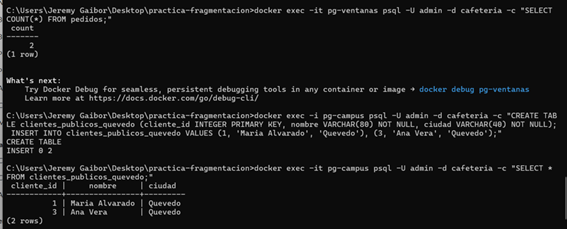
\includegraphics[width=0.6\linewidth]{imagenes/fig10_fragmento_mixto_quevedo.png}
  \caption{Fragmento mixto de datos públicos de clientes de Quevedo en \texttt{pg-campus}.}
  \label{fig:mixta_captura}
\end{figure}

Cada fragmento cumple completitud (todo cliente aparece en exactamente un
bloque público y un bloque de contacto), reconstrucción (el \texttt{JOIN} por
\texttt{cliente\_id} entre bloque público y bloque de contacto reproduce la
fila original) y disjunción (ningún cliente se repite dentro del mismo tipo de
fragmento).

% ===================== C6 =====================
\section{Vistas globales con postgres\_fdw}

Para poder consultar la información como si estuviera centralizada, se usó el
módulo \texttt{postgres\_fdw}, incluido de forma nativa en PostgreSQL, que
permite que un nodo lea tablas de otro nodo como si fueran locales
\cite{postgresfdw}. Desde \texttt{pg-campus} se definieron dos servidores
foráneos (\texttt{srv\_babahoyo} y \texttt{srv\_ventanas}), sus respectivos
\textit{user mappings}, y tablas foráneas apuntando a \texttt{pedidos} en cada
nodo remoto. Con ello se construyó la vista \texttt{pedidos\_global} como la
unión de los tres fragmentos horizontales:

\begin{lstlisting}
CREATE VIEW pedidos_global AS
SELECT * FROM pedidos
UNION ALL
SELECT * FROM pedidos_babahoyo
UNION ALL
SELECT * FROM pedidos_ventanas;
\end{lstlisting}

\begin{figure}[H]
  \centering
  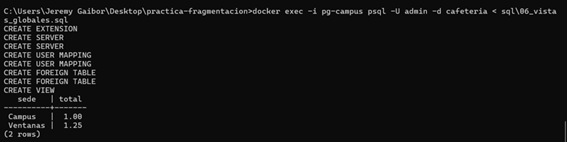
\includegraphics[width=0.6\linewidth]{imagenes/fig11_vista_global_pedidos.png}
  \caption{Reconstrucción global de \texttt{pedidos} mediante \texttt{postgres\_fdw} y \texttt{UNION ALL}.}
  \label{fig:global_pedidos}
\end{figure}

De forma análoga se construyó \texttt{clientes\_global}, uniendo por
\texttt{cliente\_id} los fragmentos públicos y de contacto de cada nodo para
reconstruir el registro completo.

\begin{figure}[H]
  \centering
  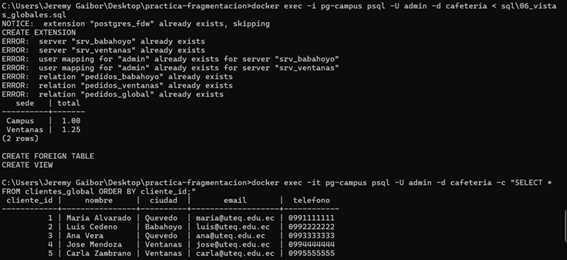
\includegraphics[width=0.6\linewidth]{imagenes/fig12_reconstruccion_vertical_clientes.png}
  \caption{Reconstrucción vertical de \texttt{clientes} mediante \texttt{clientes\_global}.}
  \label{fig:global_clientes}
\end{figure}

Ambas vistas devolvieron los mismos resultados que las consultas equivalentes
ejecutadas contra la base de datos centralizada del Paso~1, lo que confirma
que la fragmentación es transparente para el usuario final.

% ===================== C7 =====================
\section{Verificación de las propiedades de fragmentación}

Se ejecutaron tres consultas de comprobación (Listado 13) para validar que la
fragmentación horizontal cumple las tres propiedades exigidas:

\begin{itemize}
  \item \textbf{Completitud:} la suma de filas de \texttt{pedidos} en los tres
        nodos es igual al total de filas del esquema centralizado.
  \item \textbf{Disjunción:} ningún \texttt{pedido\_id} se repite entre nodos.
  \item \textbf{Reconstrucción:} la vista \texttt{pedidos\_global} devuelve
        exactamente el mismo conjunto de filas que la tabla centralizada.
\end{itemize}

\begin{figure}[H]
  \centering
  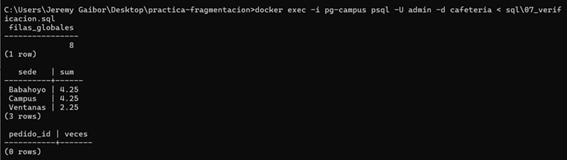
\includegraphics[width=0.6\linewidth]{imagenes/fig13_verificacion_completitud.png}
  \caption{Verificación de completitud de la fragmentación horizontal.}
  \label{fig:verif}
\end{figure}

Como evidencia adicional exigida por la rúbrica, se muestra el conteo de
filas de \texttt{pedidos} obtenido con \texttt{psql} en cada uno de los tres
nodos:

\begin{lstlisting}
docker exec -it pg-campus   psql -U admin -d cafeteria -c "SELECT COUNT(*) FROM pedidos;"
docker exec -it pg-babahoyo psql -U admin -d cafeteria -c "SELECT COUNT(*) FROM pedidos;"
docker exec -it pg-ventanas psql -U admin -d cafeteria -c "SELECT COUNT(*) FROM pedidos;"
\end{lstlisting}

\begin{figure}[H]
  \centering
  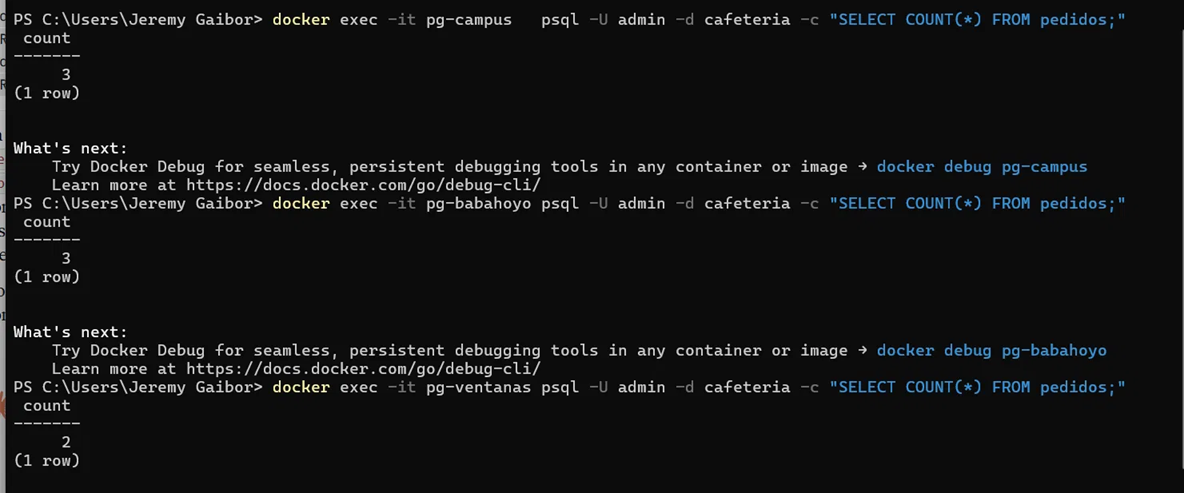
\includegraphics[width=0.6\linewidth]{imagenes/fig14_conteo_filas_nodos.png}
  \caption{Conteo de filas de \texttt{pedidos} en \texttt{pg-campus}, \texttt{pg-babahoyo} y \texttt{pg-ventanas}.}
  \label{fig:conteo}
\end{figure}

% ===================== REFLEXIÓN =====================
\section{Reflexión}

% TODO: revisa y ajusta con detalles propios de tu equipo si algo no calzó exactamente así.

Lo más difícil no fue escribir el SQL de cada fragmento, sino no perder de
vista qué fila estaba en qué nodo. Con la fragmentación horizontal de
\texttt{pedidos} fue fácil: solo hay que filtrar por \texttt{sede} y listo,
cada nodo se queda con lo suyo. El problema apareció en la fragmentación
mixta de \texttt{clientes}, donde tocaba cortar por ciudad y además por
sensibilidad del dato al mismo tiempo. Ahí sí nos tocó parar y revisar con
lápiz y papel qué \texttt{cliente\_id} iba en cada bloque, porque era fácil
dejar a alguien fuera o repetirlo en dos fragmentos por error.

\texttt{postgres\_fdw} también dio trabajo. La primera vez que intentamos
crear el servidor foráneo nos tiró error de conexión, y resultó que el
\texttt{host} que pusimos en \texttt{CREATE SERVER} no era el nombre del
contenedor tal como lo definimos en \texttt{docker-compose.yml}. Una vez
corregido eso, las vistas globales funcionaron sin más problemas y devolvían
lo mismo que la base centralizada del Paso 1, lo cual fue satisfactorio de
comprobar.

En cuanto a ventajas, lo que más se nota trabajando con esto es que cada
sede queda dueña de sus propios datos: si se cae el nodo de Ventanas, Campus
y Babahoyo siguen funcionando normal, solo se pierde acceso a los pedidos de
esa sede en particular. Eso en un sistema centralizado no pasa. También nos
gustó que separar \texttt{clientes\_publicos} de \texttt{clientes\_contacto}
deja más claro qué datos son sensibles, sin tener que aplicar permisos
columna por columna sobre una sola tabla.

Como desventaja, mantener todo esto sincronizado es más trabajo del que
parece al principio. Cualquier cambio en el esquema hay que replicarlo a
mano en los tres contenedores, y verificar que las tres propiedades
(completitud, disjunción, reconstrucción) se sigan cumpliendo no es
automático, hay que correr las consultas de comprobación cada vez. Para un
sistema pequeño como el de esta práctica es manejable, pero se nota que en
un caso real con más tablas y más nodos esto se complicaría bastante.

% ===================== REFERENCIAS =====================
\begin{thebibliography}{9}

\bibitem{ozsu}
M.~T. Özsu and P.~Valduriez, \emph{Principles of Distributed Database
Systems}, 4th ed. Cham, Switzerland: Springer Nature, 2020, doi:
10.1007/978-3-030-26253-2.

\bibitem{postgresfdw}
PostgreSQL Global Development Group, ``postgres\_fdw --- Foreign Data
Wrapper for Remote PostgreSQL Servers,'' \emph{PostgreSQL Documentation}.
[Online]. Available: \url{https://www.postgresql.org/docs/current/postgres-fdw.html}

\bibitem{docker}
Docker Inc., ``Compose File Reference,'' \emph{Docker Documentation}.
[Online]. Available: \url{https://docs.docker.com/compose/compose-file/}

\end{thebibliography}

\end{document}